\documentclass[journal]{IEEEtran}
\usepackage{subcaption} 
\usepackage{color}
\usepackage{graphicx}
\usepackage{amsfonts}
\usepackage{amssymb}
\usepackage{siunitx}
\usepackage{url}
\usepackage{comment}
\usepackage{multirow}
\newcolumntype{N}{>{\centering\arraybackslash}m{.45in}}
\usepackage{colortbl,multirow,hhline,makecell}
\usepackage[table]{xcolor}
\newcommand{\abv}[1]{{\color{red}{[#1]}}}
\newcommand{\rever}{\textcolor{blue}}
%\newcommand{\rever}[1]{{\color{blue}{[#1]}}}
\newcommand{\refazer}[1]{{\color{red}{[#1]}}}
\newcommand{\gn}[1]{{\color{red}{[#1]}}}

\usepackage{placeins}
\usepackage{float}
\usepackage[english,brazilian]{babel}
%\usepackage[english]{babel}
\usepackage[utf8]{inputenc}
\usepackage[T1]{fontenc}
\usepackage{comment}
\usepackage{xcolor}
% correct bad hyphenation here
\hyphenation{op-tical net-works semi-conduc-tor}
\usepackage{cite}

\begin{document}
\title{Cryptography Algorithms in Wearable
Communication: An Empirical Analysis}

%\author{{\bf Kristtopher~Kayo~Coelho}, {\bf Danilo~Damião}%~\IEEEmembership{Members,~IEEE,      	{\bf Alex~Borges},\\ %~\IEEEmembership{Fellow,~OSA,    {\bf Michele~Nogueira}, %~\IEEEmembership{Senior Member,~IEEE,}    {\bf Jos\'e Augusto M. Nacif},   {\bf Guevara Noubir}%,~\IEEEmembership{Life~Fellow,~IEEE}% <-this % stops a space
%\thanks{K. Coelho, D. Damião and J. Nacif is with the Science and Technology Institute, Federal University of Viçosa, Brazil} 

%\thanks{A. Borges is with the Department of Computer Science, Federal University of Juiz de Fora, Brazil.}% <-this % stops a space
%\thanks{M. Nogueira is with the Departmentof Computer Science, Federal University of Paran\'a, Brazil.}
%\thanks{G. Noubir is with the Department of Computer Science, Northeastern University, USA.
%}% <-this % stops a space
%\thanks{Manuscript received XX XX, 2018; revised August 26, 2015.}
%\vspace{-1.2cm}}

\author{%\vspace{-0.2cm}
{\bf Author 1}, {\bf Author 2}, %~\IEEEmembership{Members,~IEEE,
{\bf Author 3}, %~\IEEEmembership{Fellow,~OSA,   
{\bf Author 4}, %~\IEEEmembership{Senior Member,~IEEE,}    
{\bf Author 5}, {\bf Author 6} \vspace{-0.5cm}%,~\IEEEmembership{Life~Fellow,~IEEE}% <-this % stops a space
\thanks{Author 1, Author 2 and Author 3 are with the Institution 1. Author 4 is with the Institution 2. Author 5 is with the Institution 3. Author 6 is with the Institution 4.}
%}% <-this % stops a space
%\thanks{Manuscript received XX XX, 2018; revised August 26, 2015.
%}
\vspace{-0.5cm}}


\markboth{IEEE COMMUNICATIONS LETTERS, VOL. XX, NO. XX, MONTH Year}%
{Coelho \MakeLowercase{\textit{et al.}}: Cryptographic Algorithms in Wearable Devices}


% make the title area
\maketitle
\selectlanguage{english}

\begin{abstract}
In this letter, we assess the practical impact of lightweight block and stream cipher algorithms on power consumption and hardware resources for wearable devices that own low computational resources. Differently from the literature, we present an empirical and hardware-driven evaluation of the most representative encryption algorithms with regard to the requirements of wearable networks. We design and implement a cryptography library useful for wearable devices. Results confirm a strong correlation between the amount of logic/arithmetic operations, assembly instructions and power consumption for the two evaluated platforms, and they highlight the need to design encryption algorithms for wearable devices with high energy consumption efficiency, but strong security level similar to AES. 
\end{abstract}
\vspace{-0.3cm}
\begin{IEEEkeywords}
Wearable devices, cryptography algorithms, block cipher, stream cipher, and power consumption. 
\vspace{-0.1cm}
\end{IEEEkeywords}

\IEEEpeerreviewmaketitle

\vspace{-0.1cm}
\section{Introduction}
Market forecasts that worldwide shipments of wearable computing devices will reach 929 million in 2021, presenting as major drivers fitness and healthcare gadgets~\cite{cheung2018emerging}. Wearable computing devices are smart electronic devices (electronic device with microcontrollers) that can be incorporated into clothing, worn on the body, or implanted in the body, such as fitness trackers, smartwatches, and the ``neural dust'' implantable sensor. They have rapidly become popular due to advancements in micro and nano-electronics. Wireless communication is essential for these advancements, once it allows the connection between devices in and around the human body, including low-rate devices like pedometers and high-rate devices like augmented-reality glasses. This communication relies on different standards such as those from the IEEE 802.15 family~\cite{Li:2018} or the next generation mmWave 5G cellular. 

 Given data sensitiveness in this context, popularity and user-reliance on wearable devices, there has been an emergence of new and varied attack vectors targeting privacy intrusions, that so far cannot be addressed by classical techniques developed for the Internet applications.  In this letter, our goal lies in empirically evaluating the practical impact of the most representative lightweight cryptography algorithms with regard to the requirements of wearable networks, such as high security and low computational resources, considering energy constraints from implantable and non-implantable devices. 
 
 \rever{Most existing studies have investigated wearable network requirements either from a software perspective~\cite{kerckhof2012towards,sallam2018survey} or by simulations and analytical models~\cite{cazorla2013survey,el2017equalized}. Despite the importance of those studies, an empirical study complements them offering insights and knowledge closer to the real implementation of those cryptography algorithms, assisting then in the design of more efficient and cost-effective solutions.} To the best of our knowledge, ours is the first to follow a hardware-driven and empirical evaluation, highlighting the impacts of the hardware specificity to cryptography algorithms in wearable devices.

Our analysis targets symmetric cryptography, where the communicating wearable devices share (possibly through a pairing or authentication, and key establishment protocol) the session key used to encrypt the messages. Particularly, we focus our investigations on two different classes of symmetric lightweight encryption algorithms, as block ciphers (XTEA, XXTEA, SKIPJACK, RC2, and AES)~\cite{Moh:2015}, stream cipher (RC4). For our evaluation approach, we have designed and implemented a cryptography library useful for wireless wearable devices\footnote{Available at: [URL removed because of the double-blind review process.]% \url{https://github.com/UFV-Alumni/lib_crypto}
}. For power consumption measurements, we have designed an instrumentation circuit and integrated it in the evaluated platforms. The power consumption evaluation has followed a methodology adapted from Bessa \emph{et al.}~\cite{bessa2017jetsonleap}, that allow us to assess the power dissipation from wearable devices while they are in idle and running states. Our analysis has focused on real-life, off-the-shelf wearable platforms which consider the transmission of data and other with greater processing power abstracting communication.

Our results confirm the strong correlation between the amount of logic/arithmetic operations required to encrypt data block or stream, and their respective power consumption~\cite{mohd2018lightweight}.  Results indicate that SKIPJACK algorithm can be up to 18.76\% more efficient among the evaluated algorithms in terms of power consumption, processing up to 32x fewer instructions. It also consumes up to $\approx 3.5$x less ROM memory related to AES. Analyzing time vs. power consumption, the XTEA algorithm has a battery consumption almost 6x lower than AES. However, it is worth to highlight the high security level of AES, bringing us to the conclusion that it is necessary efforts to design encryption algorithms for wearable devices with high computational efficiency (i.e., memory usage, energy consumption) and high security level.

This letter presents the lightweight cryptography algorithms for wearable devices (Section~\ref{sec:Background}); the designed experiments and methodology (Section~\ref{sec:Methodology}); the discussion of the obtained results (Section~\ref{sec:Results}); and conclusions (Section~\ref{sec:Conclusion}).

\vspace{-0.25cm}
\section{Lightweight Cryptography Algorithms for Wearable Networks}
\label{sec:Background}

 A cryptosystem consists of a plaintext space $\mathcal{P}$, a ciphertext space $\mathcal{C}$, and a key space $\mathcal{K}$, an encryption algorithm $Enc: \mathcal{K}$ x $\mathcal{P} \rightarrow \mathcal{C}$, and a decryption algorithm $Dec: \mathcal{K}$ x $\mathcal{C} \rightarrow \mathcal{P}$. For each $k \in \mathcal{K}$ and $p \in \mathcal{P}$, it is $Dec(Enc(p)_k)_k = p$. In the communication model introduced by Shannon~\cite{shannon}, a cryptosystem provides confidentiality to the information from an attacker. Hence, a sender and a receiver communicate by a public channel, where they exchange ciphertexts. 

Symmetric key cryptography assumes a secure channel used by the communicating parties to establish a secret session key $k$, not accessible to the adversary. Given $p$, $k$, and the cryptosystem, the sender can construct the ciphertext $c$ and send it to the receiver. The receiver can reconstruct the plaintext $p$, given $c$, $k$, and the cryptosystem. Symmetric key cryptography is relevant for wearable networks, that devices and communication have severe resource constraints (e.g., energy, memory, and processing capacity), and applications demand for low response time. The attacker's main goal lies in recovering $p$ or $k$ and, according to Kerckhoff’s principle, an attacker knows the specification of the cryptosystem and has access to the ciphertext $c$. 

 While in the last decades the progress in the security cryptographic primitives was based in modeling~\cite{KatzL2014}, this work focuses on power consumption analysis of established block and stream ciphers. A block cipher is a cryptosystem with $gf(p^n)$, where $gf$ denotes the Galois field in order $n \in \mathcal{Z+}$ and plaintext $p \in \mathcal{P}$.
For each key $k$, the encryption function $Enc(p)_k$ is a permutation. In the most general case, the $\mathcal{K}$ corresponds to the set of permutations of size $2^n!$, where a single $k$ lies in a table of size $2^n$. The use of a subset of permutations is reasonable by generating a small key. To encrypt messages longer than the block size, we use a mode of operation, such as Cipher Block Chaining or Counter Mode, and integrity protection, such as Galois Counter Mode~\cite{KatzL2014}. 

 A stream cipher encrypts binary digits of a plaintext one at time. It follows an internal state $x \in \mathcal{X}$, an update function $L: \mathcal{X} \rightarrow \mathcal{X}$, and an output function $f: \mathcal{X} \rightarrow \mathcal{Z}$, where $\mathcal{Z}$ is called the keystream alphabet. An output $z \in \mathcal{Z}$ is produced at time $t$, according to $zt = f(xt)$, where $xt = Lt(x)$ and $x$ is the initial state. The stream of outputs $z_0, z_1, \ldots$ is called the keystream. Each output symbol is combined to the corresponding plaintext symbol to produce a ciphertext symbol.

 In this study, we have analyzed recent literature on wearable cryptography algorithms~\cite{cazorla2013survey, sallam2018survey, dener2018comparison}. We have chosen these algorithms based on power and processing restrictions imposed by wearable devices, considering the energy limitations of implantable and non-implantable devices. XTEA, XXTEA, SKIPJACK, RC2, and AES are block ciphers; whereas RC4 is a stream cipher. These encryption algorithms provide a security level that can handle thresholds related to low-resource, minimal area, low-memory, and low-power, being well-known as “light” algorithms. In addition to the six lightweight algorithms, briefly described in the next paragraphs, we have initially considered others, e.g., KSEED, TWOFISH, and CAST5. But, they have shown to be impractical for the current wearable device architecture due to the excessive memory use, reported from MSP430 GCC. 

The eXtension to TEA (XTEA) and the Corrected Block TEA (XXTEA) encryption algorithms employ a 128-bit key and blocks of 64-bits. XTEA operates in 64 rounds and XXTEA has a variable number of rounds. In both, permutations follow simple operations, {\em e.g.}, addition, shifting and XOR. For key recovery, the best attack reported on XTEA was a related-key differential attack on 26 out of 64 rounds. The cryptanalysis of XXTEA describes a successful chosen plaintext attack with $2^{59}$ plain-ciphertext pairs \cite{sallam2018survey}.

The SKIPJACK algorithm is a 32-round cipher which applies two distinct rules labeled as A and B. These rules are applied interleaved as A, B, A, B per 8 rounds. Permutations comprise of shifts and Feistel's, which use 32 of the 64 bits from the secret key per permutation. Despite the controversy around SKIPJACK design, cryptanalysis point out a resistance for attacks of $2^{48}$, using at least $2^{34}$ plaintexts~\cite{biham2005cryptanalysis}. As SKIPJACK, RC2 works on 64-bit blocks and allows a variable key size. It follows the key expansion and encryption steps. Key expansion can extend any key size, in the range of 1 to 128 bytes, up to a 128-byte key. Encryption performs permutations based on a substitution table. Estimates to retrieve a secret key are proportional to the effort for analyzing about $2^{4r}$ (for $r$ = 16) chosen plaintexts~\cite{knudsen1998design}.

The Advanced Encryption Standard (AES) algorithm has become the primary choice for various security services due to its strong defense against known attacks. The best known attacks against AES are slightly faster than brute-force and require $2^{126.2}$ operations to recover an AES-128 key. In~\cite{nasser2016aes}, the authors presented an optimized version of AES for devices with low computational capacity and memory resources, while still providing low power consumption. 

RC4 is a stream cipher and it comprises of a Key Scheduling Algorithm (KSA) and a Pseudo-Random Generation Algorithm (PRGA). KSA transforms a random key in an initial permutation, whereas PRGA uses this initial permutation to generate a pseudo-random output sequence. Cryptographic transformations applied by the algorithm are linear and simple, using permutations and sums of integer values. However, secure use of RC4 is non-trivial as experienced with Wi-Fi WEP. However, the recovery requires a complex process of about $2^{13}$ algorithm operations for 256-bit key~\cite{son2019fast}.

\vspace{-0.25cm}
\section{Experiments and Methodology}
\label{sec:Methodology}

 In this work, the experiments rely on two platforms: $(i)$ wearable devices from the Shimmer platform, model 2R and $(ii)$ a Teensy\texttrademark~3.2 microcontroller. The Shimmer devices are equipped with a MSP430 F1611 microcontroller, 16-bit RISC architecture. Each wearable device contains 48KB flash memory and 10KB RAM. These devices sense vital signs and movements from users by accelerometers, magnetometers, and gyroscope, and transmit them to a coordinator device ({\em e.g.}, a smartphone) through wireless communication. These low-power wireless devices run TinyOS, a Real-Time Operating System (RTOS). The Teensy platform is equipped with an ARM\textsuperscript{\textregistered} Cortex\textsuperscript{\textregistered}-M4 of 72 MHz CPU and 32-bit architecture. This device also contains a 256KB flash memory and 64KB RAM memory. For Teensy, the algorithms were implemented in C language and deployed using the Arduino interface.

 We measure power consumption in different states ({\em i.e.}, idle, and run). At a glance, we set up the devices to the desired state and continuously monitor it. The devices are automatically placed in a low-power mode when the task queue is empty (\textit{idle} state). Hence, we are able to measure the device power consumption in this state. Finally, to analyze the wearable on the run state, we set up the device to continuously perform a cryptography task --- on 64-bits data blocks --- using one of the aforementioned cryptography algorithms on both platforms, {\em run} state). In the Shimmer platform, {\em run} state, we consider the cost of encrypted data transmission. Finally, unless we tell otherwise, at each state we perform 2,000 samples and present mean confidence interval of 95\%.

We have designed and assembled a circuit for power consumption measurement adapted from~\cite{bessa2017jetsonleap}. The circuit comprises of a low-cost data acquisition board (DAQ - ADALM1000) connected to a wearable, a 0.10~\si{\ohm} resistor, and a computer (Figure~\ref{fig:circuit}). We use Active Learning Interface for Circuits and Electronics (ALICE) software to acquire voltage measurements from both terminals of the resistor which are connected to channels CH\_A and CH\_B of the DAQ. The voltage can be easily transformed to current following the law of Ohm, $V = R$ x $I$, since the resistance value is known. 
To make comparisons, we calculate the power consumption by multiplying the current to the voltage. Then, power consumption follows: 
$P = ((\mbox{CH\_A} - \mbox{CH\_B}) / 0.10) * V $ mW.

\begin{figure}[!htb]
 \vspace{-0.3cm}
 \centering
 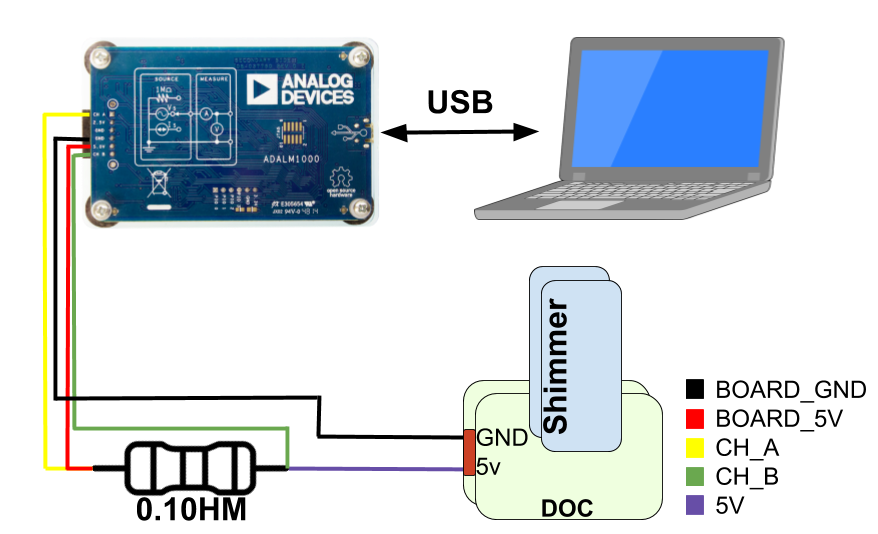
\includegraphics[scale=0.19]{Figures/circuit.png}
 \caption{Power consumption measurement}
 \label{fig:circuit}
 \vspace{-0.3cm}
\end{figure}

DAQ delivers a maximum sampling rate of 100 ksps (kilosamples per second). Therefore, we calculate power consumption, mean, and the total consumption time for the algorithms in each analyzed state of wearable devices. Also, the computational complexity of the algorithms is of great relevance because power consumption bottlenecks occur during data processing and transmission. Hence, we also consider the size of machine code, when it represents a large share of the hardware resource consumption.

We also count the number of Assembly instructions using the Godbolt online compiler and a manual process known as Table Test. The Godbolt compiler converts programs from several languages into Assembly code. For the experiment, we use the MSP430 GCC compiler version 5.3.0 for Shimmer platform and AVR GCC version 4.6.4 for Teensy platform, both without optimization directives. Then, we convert the code to Assembly code. Next, using the Table Test, we have counted the final number of Assembly instructions.

 Similarly, we also analyze the main operations in each cryptography algorithm. The considered operations are {\em shift left, shift right, and, or, not, xor, sum, subtraction}, and {\em multiplication}. We enumerate all these logical and arithmetic operations when we want to confirm if the number of operations can be directly correlated with the final performance and power consumption of each algorithm implementation~\cite{mohd2018lightweight}. Furthermore, since wearable devices are severely constrained in computational resources, and implantable devices have hard limitations for replacement, we analyze the amount of memory the implementation of each algorithm requires. We derive this information to memory consumption (ROM and RAM separately) of each cryptography algorithm using MSPGCC compiler for Shimmer platform and AVR GCC for Teensy platform~\cite{cazorla2013survey}. To ensure equivalence between measurements, we disregard the overhead produced by TinyOS on the Shimmer platform. Hence, we can assert that the presented data refers exactly to each algorithm.

\vspace{-0.3cm}
\section{Results}
\label{sec:Results}

 Power consumption is one of the critical factors in the design and development of wearable networks for both high-end and low-end embedded devices. Therefore, a comprehensive power efficiency analysis, considering all possible factors is of great relevance. A Power State Machine (PSM) represents the possible states of a device, and a transition between two states means power cost and delay.
Thus, low power states have a longer delay between transitions for {\em run} states. The transition time is presented in~\cite{goraczko2008energy}. The time for other transitions is considered insignificant and it is not represented in PSM.

 Figure~\ref{fig:PSM_geral} represents the PSM of the evaluated devices. In the {\em idle} state, the employed platforms run automatically under low energy consumption, being attractive because they manage themselves the different levels of suspension and interruptions, which makes easier for the developer. The figure also presents the average power consumption for each cryptographic algorithm and evaluated state and the transition time between states. Thus, we highlight the SKIPJACK algorithm, that improves energy efficiency in 18\% compared to AES.

\begin{figure}[tbh]
 \vspace{-0.3cm}
 \centering
 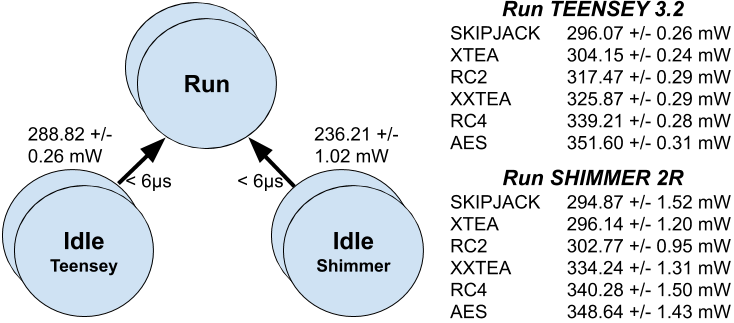
\includegraphics[scale=0.25]{Figures/PSM_Geral.png}
 \caption{ Wearable device power state machine (PSM)}
 \label{fig:PSM_geral}
 \vspace{-0.3cm}
\end{figure}

\begin{figure*}[!t]
 \vspace{-0.5cm}
\centering
 \begin{subfigure}[b]{0.35\textwidth}
  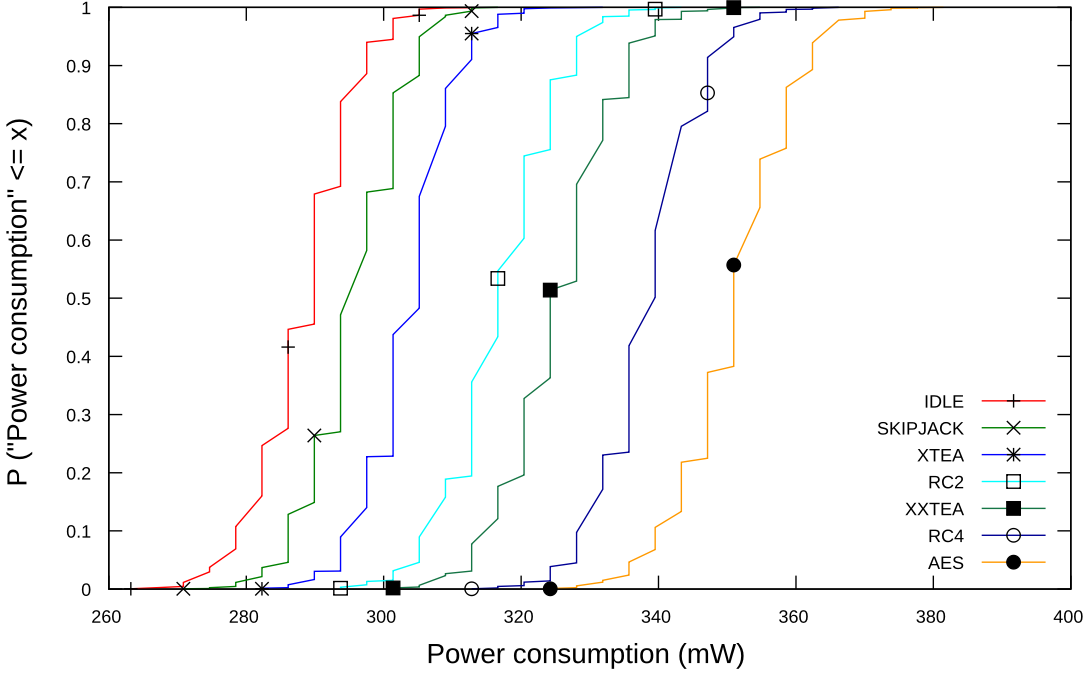
\includegraphics[width=0.9\textwidth]{Figures/cdf_Teensy.png}
  \caption{ Power consumption per state Teensy 3.2}
  \label{fig:cdf_Teensy}
 \end{subfigure}
 %\hspace{10mm}
 \begin{subfigure}[b]{0.35\textwidth}
  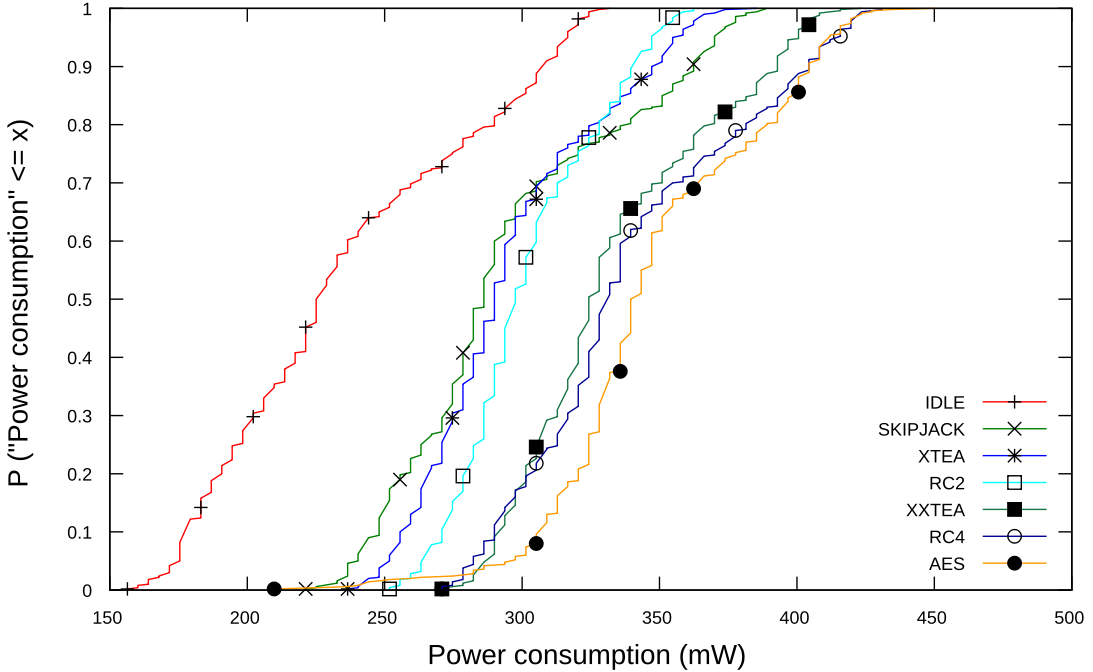
\includegraphics[width=0.9\textwidth]{Figures/cdf_zig.png}
  \caption{ Power consumption per state Shimmer 2R}
  \label{fig:cdf_zig}
 \end{subfigure}
 \vspace{-0.2cm}
 \caption{Power consumption in milliwatts on the {\em run} state}
 \label{fig:cdf}
 \vspace{-0.45cm}
\end{figure*}

 The {\em run} state asymptotically dominates energy consumption. The analysis of power consumption for the Shimmer platform includes cryptographic processing and radio data transmission. With the Teensey platform, we have excluded the transmission operation and we can observe a similarity in the allusive behavior to the energy consumption of the cryptographic algorithms. Figure~\ref{fig:cdf} shows the behavior of the evaluated algorithms in both platforms through the Cumulative Distribution Functions (CDFs). Figure~\ref{fig:cdf_Teensy} illustrates the results for the Teensy platform, and Figure~\ref{fig:cdf_zig} presents results for the Shimmer platform.

 The computational cost of logical and arithmetic operations has a direct effect on processing time and wearable device power consumption. Table~\ref{tab:comp} shows the number of operations for each evaluated algorithm and their respective complexity. The count is relative to the encryption function, once the wearable device performs this function, but not decryption. Thus, power consumption has a direct correlation with the number of operations. Another correspondence observed is the proportionality of ROM/RAM occupancy between the algorithms, $\approx11$\%. In addition to finding a ROM memory consumption about $\approx3.5$x higher of AES in relation to SKIPJACK, considering the Shimmer platform.

\begin{table}[h!]
\scriptsize
\centering
 \setlength\tabcolsep{7.7 pt} 
\vspace{-0.1cm}
\caption{ Computational complexity vs. memory consumption}
\vspace{-0.2cm}
\begin{tabular}{l|c|ccll}
\hline

\multirow{3}{*}{ALGORITHM} & \multirow{3}{*}{\begin{tabular}[c]{@{}c@{}}COMPLEXITY\end{tabular}} &\multicolumn{4}{c}{\begin{tabular}[c]{@{}c@{}} MEMORY CONSUMPTION (BYTES)\end{tabular}}\\ \cline{3-6} 
          &                 & \multicolumn{2}{c|}{ Shimmer 2R}                               & \multicolumn{2}{c}{ Teensy 3.2}    \\ \cline{3-6} 
            &               & \multicolumn{1}{c|}{ ROM}  & \multicolumn{1}{c|}{ RAM}  & \multicolumn{1}{c|}{ ROM}  &  RAM  \\ \hline
SKIPJACK    & $O(1)$        & \multicolumn{1}{c|}{ 6,834}        & \multicolumn{1}{c|}{ 608}          & \multicolumn{1}{l|}{ 13,892}       &  4,584 \\
XTEA        & $O(1)$        & \multicolumn{1}{c|}{ 6,772}        & \multicolumn{1}{c|}{ 612}          & \multicolumn{1}{l|}{ 13,360}       &  4,620 \\
RC2         & $O(1)$        & \multicolumn{1}{c|}{ 6,786}        & \multicolumn{1}{c|}{ 726}          & \multicolumn{1}{l|}{ 14,028}       &  4,828 \\
XXTEA       & $O(n)$        & \multicolumn{1}{c|}{ 7,064}        & \multicolumn{1}{c|}{ 604}          & \multicolumn{1}{l|}{ 13,456}       &  4,556 \\
RC4         & $O(n)$        & \multicolumn{1}{c|}{ 6,994}        & \multicolumn{1}{c|}{ 604}          & \multicolumn{1}{l|}{ 13,348}       &  4,556 \\
AES         & $O(1)$        & \multicolumn{1}{c|}{ 24,068}       & \multicolumn{1}{c|}{ 1,978}        & \multicolumn{1}{l|}{ 14,048}       &  4,812 \\ \hline
\end{tabular}
\label{tab:comp}
\vspace{-0.5cm}
\end{table}

 Table~\ref{tab:instr} displays information about the amount of logical/arithmetic operations and assembly instructions performed by each cryptographic algorithm. This allows us to draw a direct correlation between these parameters and energy consumption. Hence, we observe that the SKIPJACK algorithm performs fewer operations and, thus, fewer instructions ($\approx 32$x), requiring less hardware performance and less energy, particularly, when compared to AES.

\begin{table}[h!]
\centering
\scriptsize
\setlength\tabcolsep{3pt} % default value: 6pt
\vspace{-0.1cm}
\caption{ Logic/arithmetic operations vs. assembly instructions}
\vspace{-0.2cm}
\begin{tabular}{l|c|c|c|c|lc}
\hline
\multirow{3}{*}{ALGORITHM} & 
\multirow{3}{*}{\begin{tabular}[c]{@{}c@{}}\#LOGICAL/\\ARITHMETC\\OPERATIONS\end{tabular}} & \multirow{2}{*}{\begin{tabular}[c]{@{}c@{}}NUMBER\\OF\\ROUNDS\end{tabular}} & \multicolumn{2}{c|}{Shimmer 2R}                                      & \multicolumn{2}{c}{ Teensy 3.2}\\ \cline{4-7} 
\multicolumn{1}{c|}{}             &               &                                        &\begin{tabular}[c]{@{}c@{}}MAIN\\LOOP\end{tabular} & \begin{tabular}[c]{@{}c@{}}TOTAL\\\#INSTR.\end{tabular} & \multicolumn{1}{c|}{\begin{tabular}[c]{@{}c@{}}MAIN\\LOOP\end{tabular}} & \begin{tabular}[c]{@{}c@{}}TOTAL\\\#INSTR.\end{tabular} \\ \hline
SKIPJACK    & 496       & 32        & 665       & 760       & \multicolumn{1}{l|}{1,680}        & 1,908  \\
XTEA        & 576       & 32        & 1,184     & 1,206     & \multicolumn{1}{l|}{4,256}        & 4,329  \\
RC2         & 804       & 16        & 1,550     & 1,645     & \multicolumn{1}{l|}{6,832}        & 7,075  \\
XXTEA       & 1,490     & 12        & 5,748     & 5,776     & \multicolumn{1}{l|}{15,936}       & 16,034 \\
RC4         & 1,992     & 8         & 400       & 10,677    & \multicolumn{1}{l|}{1,088}        & 30,703 \\
AES         & 2,704     & 9         & 21,636    & 24,117    & \multicolumn{1}{l|}{48,087}       & 54,552 \\ \hline
\end{tabular}

\label{tab:instr}
\vspace{-0.2cm}
\end{table}

Taking as a basis the cryptanalysis presented in Section~\ref{sec:Background}, we analyze the tradeoff between power consumption and the  security level for each algorithm. SKIPJACK and AES are the two extremes. SKIPJACK is the most power efficient; whereas AES has the highest power consumption. However, AES presents the highest security level. 

We could also predict the battery lifetime for the devices, as shown in Table~\ref{tab:battery_life}. We consider an internal battery of 450~mA in the Shimmer platform and a demanding scenario, in which the device performs a data transmission per minute. It is estimated that the device can respond uninterruptedly for up to 67 hours using XTEA as a cryptographic algorithm. This means that the choice of the algorithm can directly influence up to $\approx 5.9$x the battery lifetime.

\begin{table}[h!]
\scriptsize
\centering
\setlength\tabcolsep{7pt} % default value: 6pt
\vspace{-0.1cm}
\caption{Battery life expectancy}
\vspace{-0.2cm}
\begin{tabular}{l|c|c|c}
\hline
ALGORITHM  & TIME (S) & \begin{tabular}[c]{@{}c@{}}AVERAGE\\CONSUMPITION (mA) \end{tabular} & \begin{tabular}[c]{@{}c@{}}BATTERY\\LIFE (HH:MM) \end{tabular}\\ \hline
SLEEP MODE & ------             & 0.0011                    & -----\\
SKIPJACK   & 33.00              & 58.974                    & 40:55\\
XTEA       & 12.93              & 59.228                    & 67:00\\             
RC2        & 14.62              & 60.554                    & 62:58\\          
XXTEA      & 39.64              & 66.848                    & 33:24\\              
RC4        & 59.47              & 68.056                    & 24:17\\
AES        & 138.00             & 69.728                    & 11:34\\ \hline
\end{tabular}
\vspace{-0.3cm}
\label{tab:battery_life}
\end{table}

\vspace{-0.2cm}
\section{Conclusion}
\vspace{-0.1cm}
\label{sec:Conclusion}

In this letter, we have investigated block and stream ciphers in terms of resource usage and power consumption for end-to-end wearable devices secure communications. We have performed a hardware-driven power consumption measurement evaluation under two platforms with constrained resources. The SKIPJACK algorithm exhibits the best performance for power consumption and the second least memory usage. The XTEA algorithm presents the longest battery lifetime. However, differently from AES, SKIPJACK and XTEA have potential vulnerabilities pointed out in the literature. Hence, despite the computational and energetic efficiency of SKIPJACK and XTEA for the evaluated wearable devices, AES still presents a high security level, leading us to the conclusion that there is still a need to design encryption algorithms for wearable devices with high energy consumption efficiency and security level similar to AES.

\vspace{-0.4cm}
\selectlanguage{english}
\bibliographystyle{IEEEtran}
\bibliography{bibtex/bib/Letter.bib}
\vspace{-0.3cm}
\end{document}